\documentclass{aleph-revista}

\usepackage{tikz}           
\usepackage{aleph-comandos} 
\usepackage{multicol}    
\usepackage{indentfirst}
\usepackage{cleveref}
\usepackage{circuitikz}
\usepackage{graphicx}
\usepackage{listings}
\usepackage{xcolor}
\usepackage{tikz-dimline}
\usepackage{steinmetz}
\usetikzlibrary{arrows,calc,patterns,decorations.markings,arrows.meta,quotes}

\definecolor{commentgreen}{RGB}{2,112,10}
\definecolor{eminence}{RGB}{108,48,130}
\definecolor{weborange}{rgb}{0.58,0,0.82}
\definecolor{frenchplum}{RGB}{129,20,83}

\definecolor{tabred}{RGB}{214, 39, 40}
\definecolor{tabblue}{RGB}{31, 119, 180}
\definecolor{tabgreen}{RGB}{44, 160, 44}

\lstset {
    language=Python,
    frame=tb,
    tabsize=4,
    showstringspaces=false,
    numbers=left,
    upquote=true,
    commentstyle=\color{commentgreen},
    keywordstyle=\color{eminence},
    stringstyle=\color{red},
    basicstyle=\small\ttfamily,
    emphstyle={\color{blue}},
    escapechar=\&,
    classoffset=1,
    otherkeywords={>,<,.,;,-,!,=,~},
    morekeywords={>,<,.,;,-,!,=,~},
    keywordstyle=\color{weborange},
    classoffset=0,
}
% \graphicspath{{figures/}}

\titulo{Exercício Computacional 02}
\tituloingles{Método dos Momentos}

\autor{%
  Natanael Magalhães Cardoso\textsuperscript{1}
}

\institucion{
\textsuperscript{1}%
  n$^{o}$ USP: 8914122
}

\fecha{31 de julho de 2021}

% \abstract{
%   Este relatório mostra uma solução computacional de um problema do eletromagnetismo com um algorítmo de diferenciação numérica, o Método das Diferenças Finitas. Aqui são expostos dois problemas onde as equipotenciais, as linhas de campo elétrico e o valor da resistência são calculados.
% }

\begin{document}
\membrete

\vspace{1em}


\section{Matriz de Capacitâncias $[C']_3$}
% \subsection{Hipóteses}
% \begin{enumerate}
%   \item Pelos valores da Tabela \ref{tab:dados}, a seguinte relação é estabelecida: $2a \ll \min(d, D, \mathcal{H}_k)$, onde $a$ é o raio de cada linha de transmissão, $\mathcal{H}_k$ é a altura da linha $k$ em relação ao solo, $D$ é a distância horizontal entre as linhas e $d$ é a distância vertical entre as linhas. Como o diâmetro da linha é $\approx 50$ vezes menor que a menor grandeza mensionada, as linhas de transmissão serão simplificados por linhas de carga imagens (retas) usando o método das imagens.
%   \item Um fio descarregado tem influência desprezível sobre o potencial produzido pelo outro.
%   \item As linhas de carga são uniformimente carregadas com cargas $Q_i$ e $-Q_i$.
% \end{enumerate}

\subsection{Inspeção da representação computacional do sistema}
A implementação deste algorítmo representa a geometria do problema por uma matriz. Antes de executá-lo para calcular algum valor, é importante verificar se a geometria do sistema está devidamente representada pela matriz. O diagrama da Figura \ref{fig:matrix} mostra a forma geral da matriz, no painel à esquerda, e os limites das posições dos corpos, nos painéis à direita.


\newpage

\begin{figure}[!h]
  \centering
  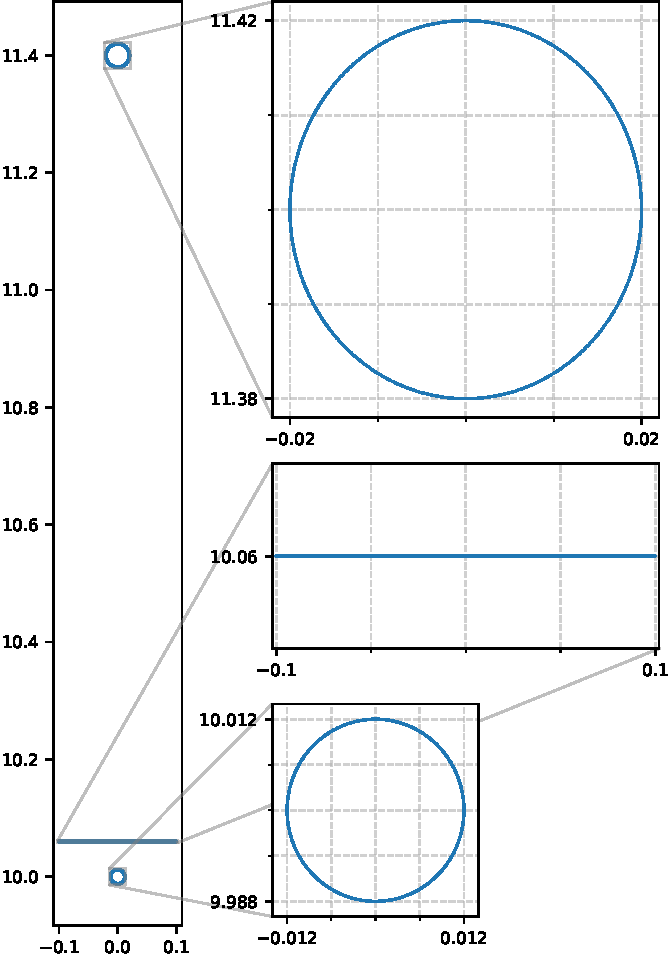
\includegraphics[width=\textwidth]{figures/matrix_plot.pdf}
  \caption{Visualização da matriz do sistema. O painél da esquerda mostra a geometria da matriz do sistema e os da direita mostram os corpos 1, 2 e 3 (de baixo para cima) em escala aumentada. Os pontos azuis indicam os cilindros de raio $b=1\cdot 10^{-4}$.}
  \label{fig:matrix}
\end{figure}

\newpage


\subsection{Calibração do raio dos cilindros de discretização}
Nesta implementação do algorítmo do Métodos dos Momentos, os corpos são discretizados por pequenos cilindros. A acurácia do resultado numérico calculado (da aproximação calculada) pelo algorítmo é tão melhor quanto menor for o tamanho deste raio. Sendo assim, uma calibração do raio foi feita para validar que a aproximação calculada seja suficientemente próxima ao valor real. Nesta calibração, é ajustado um valor para o raio tal que o erro percentual, calculado a partir da equação \eqref{eq:erro}, entre o valor estimado e o teórico seja menor que 0.5\%. A Figura \ref{fig:calibration} mostra este erro percentual em função do raio dos cilindros de discretização. O menor erro percentual obtido foi de 0.0205\% para o raio de discretização $b=5\cdot 10^{-5}$.

\begin{equation}\label{eq:erro}
  \text{Erro percentual} = \left|\frac{C_{teo} - C_{calc}}{C_{teo}}\right|
\end{equation}

\begin{figure}[!h]
  \centering
  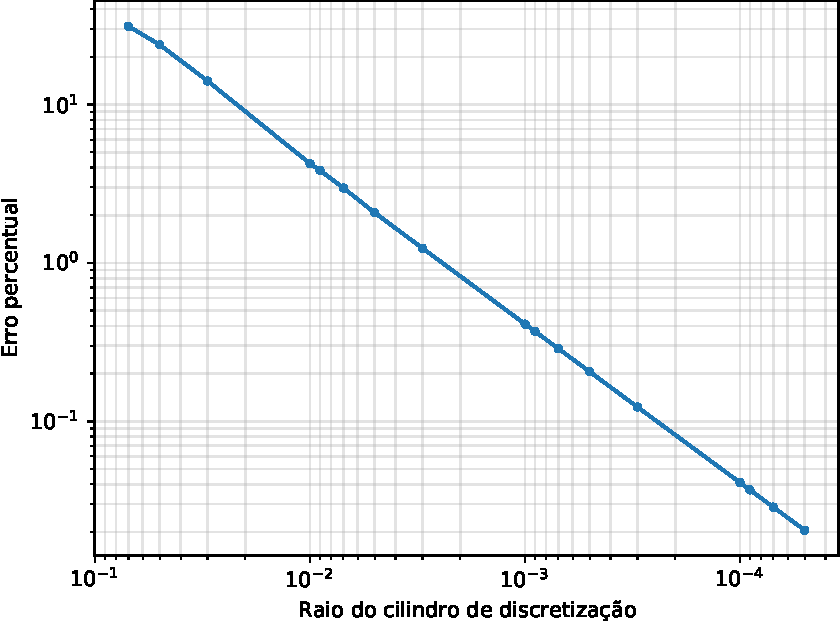
\includegraphics[width=0.95\textwidth]{figures/calibration}
  \caption{Gráfico log-log (com o eixo $x$ invertido) do erro percentual entre o valor da capacitância no corpo 1 calculado pelo algorítmo e o valor teórico em função do raio do cilindro de discretização.}
  \label{fig:calibration}
\end{figure}




